\chapter{RESULTADOS DE 2 Y 3 QUBITS}
\janote{\textbf{Idea principal del capítulo:} los resultados gritan que los 
canales PCE sí se pueden caracterizar, pero nos hace falta LA idea (la de 
Francois, jajaja) para poder formalizar la caracterización general. Para mientras,
tenemos un listado de características que tienen sustento en los resultados
numéricos.}
\section{Introducción}

\section{Resultados}
En esta sección vamos a presentar los canales cuánticos PCE de 2 y,
parcialmente, los de 3 qubits 
encontrados con el método numérico descrito en la sección 
\ref{sec:ch2_solucionNumerica}; también vamos a discutir la complejidad 
computacional del problema de 3 qubits y justificar porqué no lo estudiamos completo.
Se encontraron las siguientes proporciones de canales cuánticos PCE a 
operaciones PCE: $67:32,768$ para 2 qubits, y $716:83,456$ para 
3 qubits. Recordemos que la diferencia entre una operación y un canal cuántico PCE
es que el último satisface la condición de completa positividad y, por tanto, 
es una operación que representa la evolución física de un sistema. 
Las proporciones de canales cuánticos PCE a operaciones PCE son un indicio 
de lo restrictiva que es la condición de completa positividad para que 
una operación que borra las componentes de Pauli sea un canal cuántico.

Para decidir qué subconjunto de las operaciones PCE de 3 qubits puede analizar
nuestro método numérico también es necesario conocer el número 
de operaciones PCE en función del número de componentes 
de Pauli invariantes. Las operaciones PCE están caracterizadas 
por los $4^n$ elementos $\taus$. No obstante, por definición, 
para preservar la traza de la matriz de densidad, $\tau_{0,\ldots,0}=1$.
Entonces hay sólo $4^n-1$ elementos $\taus$ que pueden tomar los valores de 1 o 0.
La cantidad de operaciones PCE de $n$ qubits que dejan invariantes $k$ componentes 
de Pauli es igual al número de formas distintas de asignar el valor 1
a $k-1$, de los $4^n-1$, elementos $\taus$, y 0 al resto al resto de ellos; 
es decir, el coeficiente binomial $\binom{4^n-1}{k-1}$. Por las propiedades
del coeficiente binomial, el número de operaciones PCE que dejan invariantes 
$k$ componentes de Pauli es igual al número de operaciones que dejan $4^n-k$
componentes de Pauli. 

El tiempo de cómputo es el obstáculo que le impide a nuestro método numérico
poder analizar todas las operaciones PCE de 3 qubits. 
El número total de operaciones PCE para el caso 
de 3 qubits es de alrededor de $9\times10^{18}$. Supongamos por un momento
que contamos con una computadora promedio de un estudiante guatemalteco 
de física que tiene memoria RAM ilimitada y que puede analizar 
la completa positividad a una tasa de 1000 operaciones PCE de 
3 qubits por segundo. Si además asumimos que la complejidad 
algorítmica del problema es lineal, a esa computadora le tomaría, aproximadamente, 
$1/5$ de la edad del universo (¡¡$270$ millones de años!!) 
analizar todas las operaciones PCE de 3 qubits. En resumen, aunque 
la memoria RAM disponible fuese infinita, es imposible encontrar con 
nuestro método numérico todos los canales cuánticos PCE de 3 qubits
por el tiempo de cómputo. 

Por otra parte, aún delimitando la entrada del método numérico a 
únicamente las operaciones PCE de 3 qubits que dejan invariantes 
$k$ componentes de Pauli, para la computadora a nuestra disposición 
supondría un problema de memoria RAM a partir de $k=5$ hasta $k=60$.
En la gráfica de la \Fref{fig:memory_usage_3Q_5c} mostramos el uso de la 
memoria RAM de nuestro método numérico para analizar las operaciones 
PCE de 3 qubits que dejan invariantes 5 componentes de Pauli, 
en función de la cantidad de matrices. 
Se realizó un ajuste lineal a los datos para estimar 
el orden de magnitud de la cantidad de memoria necesaria para analizar todas 
las operaciones PCE de 3 qubits que dejan invariantes 5 componentes de Pauli.
La función $RAM(n)$ estima que se necesitan aproximadamente 
$1.1$ TB de memoria para analizar las 595,665 operaciones. 
Es por esta razón que, para 3 qubits, estudiamos sólo las operaciones PCE 
que dejan invariantes desde 1 hasta 4 y desde 61 hasta 64 
componentes de Pauli.
\begin{figure}
  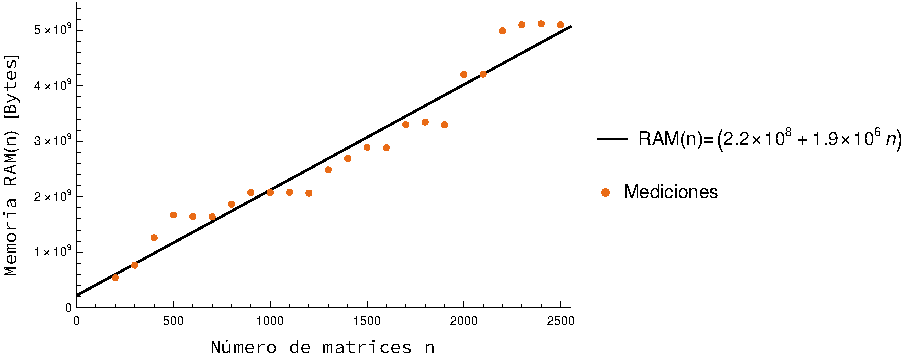
\includegraphics[width=\textwidth]{memory_usage_3Q_5c}
  \caption{Memoria RAM utilizada por el método numérico para analizar las
  operaciones PCE de 3 qubits que dejan invariantes 5 componentes de Pauli.
  El método numérico fue ejecutado en Wolfram Mathematica 12.1, operando
  en una PC con procesador Intel® Xeon(R) E-2246G~@~3.60GHz×12 
  y sistema operativo Ubuntu 20.04.3 LTS. \ep}
  \label{fig:memory_usage_3Q_5c}
\end{figure}

En la \Tref{tab:2qubitsPCEChannel1sAnd0s} (ir al apéndice A) mostramos
todos los canales cuánticos PCE de 2 qubits y en la tabla 
\Tref{tab:3qubitsPCEChannel1sAnd0s} mostramos sólo 
70 de los 716 canales cuánticos PCE de 3 qubits que dejan invariantes 
1, 2, 4 y 64 componentes de Pauli. Poner todos los canales PCE de 3 
qubits que se encontraron ocuparía demasiadas páginas y no aportan 
información extra para fines de la discusión de resultados.
Igualmente, al lector que interesado en los resultados completos,
lo invitamos a revisar el archivo de Mathematica mencionado 
al final de la sección \ref{sec:ch2_solucionNumerica}. 
En las tablas del apéndice A se muestran
(a) los valores de los elementos $\tau_{ij}$ o $\tau_{ijk}$ (1 o 0) que caracterizan 
a una operación PCE, según la definición en \eqref{eq:PCE_definition},
y (b) el número de componentes de Pauli que el canal PCE
deja invariantes. Las listas de 1's y 0's hacen difícil de escudriñar
las características que comparten todos los canales PCE.
Además, hasta ahorita no contamos con una representación geométrica, 
como la de la esfera de Bloch para 1 qubit, con la cual puedan visualizarse 
las operaciones PCE y desarrollar intuición sobre ellas.
Por lo tanto, es necesario introducir una herramienta
que permita visualizar los resultados de la \Tref{tab:2qubitsPCEChannel1sAnd0s}
de una forma más sencilla e intuitiva. Hablaremos de una herramienta geométrica
en la próxima sección.

\section{Una representación geométrica}\label{sec:ch3_geometric_representation}
%\esqueleto{Motivados en lo intricado de inferir qué características 
%comparten los canales PCE a partir de las listas de 1's y 0's, se nos ocurrió 
%una forma de representar geométricamente a las operaciones PCE que hace
%más sencillo el análisis de resultados.}

En la sección anterior vimos que los resultados de los canales PCE,
presentados como listas de 1's y 0's 
de de los elementos $\taus$ en las tablas \ref{tab:2qubitsPCEChannel1sAnd0s} y 
\ref{tab:3qubitsPCEChannel1sAnd0s}, no hacen sencilla la tarea de analizar 
las propiedades que comparten los canales cuánticos PCE. Por eso, 
buscamos una representación de las operaciones PCE que haga más fácil 
e intuitiva la identificación de las características de un canal PCE. 
Lo que buscamos es una herramienta como la esfera de Bloch, 
una representación geométrica con la cual es posible asimilar las listas 
de 1's y 0's de los canales PCE de 1 qubit en la \Tref{tab:1qubit_PCE}.  
En esta sección vamos introducir la representación de las figuras PCE 
y a presentar de nuevo los resultados de la sección anterior 
utilizando esta nueva representación de las operaciones PCE.

%\esqueleto{La figura asociada con una operación PCE de 1 qubit 
%es una columna de 
%cuadritos.. bla bla y con figuritas, haciendo referencia a lo que se resolvió 
%en el capítulo anterior, etc.}

En la \Fref{fig:PCE_figs} introducimos las figuras PCE para representar 
a las operaciones PCE. Mostramos la figura PCE de la operación identidad
de 1, 2 y 3 qubits, una operación PCE con todos los elementos 
$\tau_i$, $\tau_{ij}$ y $\tau_{ijk}$, respectivamente, iguales a 1. En una 
figura PCE, la posición de cada cuadro o cubo está asociada con los índices 
$j_1,\ldots,j_n$ de los elementos $\taus$ de una operación PCE.  
Los cuadros pintados de negro, en figuras PCE de 1 y 2 qubits, 
o cubos pintados de rojo, azul o verde, en una figura PCE de 
3 qubits, están asociados con los elementos $\tau_{k_1,\ldots,k_n}$ iguales a 1; y
los cuadros o cubos no pintados están asociados con los $\tau_{l_1,\ldots,l_n}$
iguales a 0 de una operación PCE. 
La razón por la que las figuras PCE de 3 qubits tienen colores y las de 1 y 2 
qubits no, es únicamente para servir de ayuda visual.
Los cubos con posiciones $(i,0,0)$, $(0,j,0)$ y $(0,0,k)$ se pintan de rojo; 
los cubos con posiciones $(i,j,0)$, $(0,j,k)$ y $(i,0,k)$ se pintan de azul;
y los cubos con posición $(i,j,k)$ se pintan de verde. 
\begin{figure} % {{{
	\centering
	\begin{subfigure}[b]{0.3\textwidth}
		\centering
		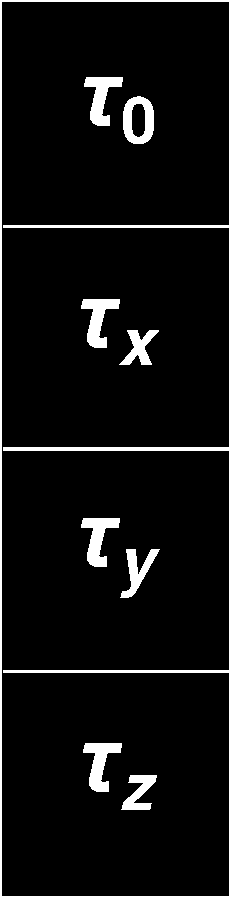
\includegraphics[height=3cm]	{tablero_1qubit}
		\caption{}
	\end{subfigure}
	\hfill
	\begin{subfigure}[b]{0.3\textwidth}
		\centering
		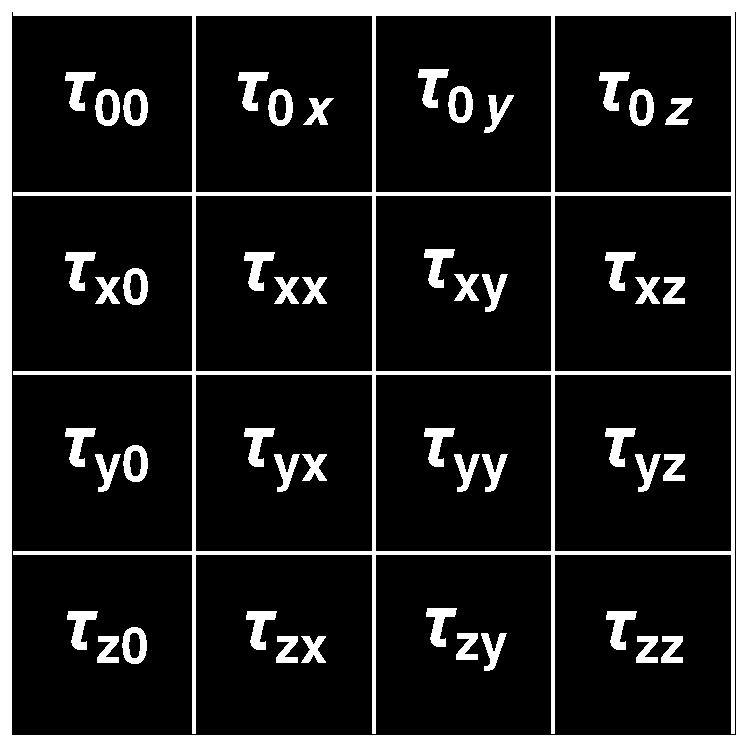
\includegraphics[height=3cm]{tablero_2qubits}
		\caption{}
	\end{subfigure}
	\hfill
	\begin{subfigure}[b]{0.3\textwidth}
		\centering
		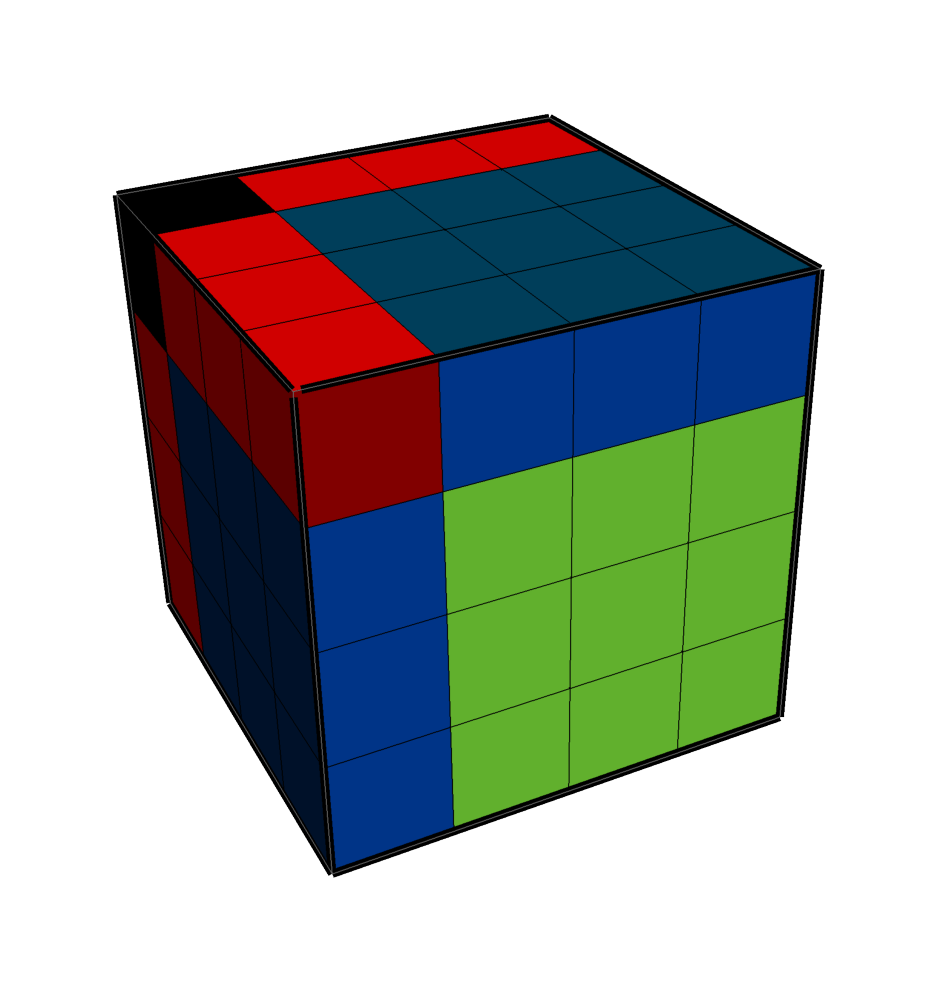
\includegraphics[height=3cm]{cubo_3qubits}
		\caption{}
	\end{subfigure}
	\caption{De izquierda a derecha se muestran las figuras PCE de la operación
	identidad de 1, 2 y 3 qubits. En esta representación los índices $j_1,\ldots,j_n$
	de los elementos $\taus$ de la operación PCE	están asociados con una posición 
	en la figura PCE respectiva. Si la posición $j_1,\ldots,j_n$ en 
  la figura PCE está pintada, entonces el elemento asociado $\taus$ es 
  igual a 1, y si la posición no está pintada (en blanco), entonces el elemento 
  asociado $\taus$   es igual a 0. \ep}
	\label{fig:PCE_figs}
\end{figure} % }}}

%\esqueleto{Para una operación PCE de 2 qubits, los dos índices en las $\tau$
%sugieren que ahora la figura asociada debería ser de dos dimensiones. Así, 
%los tableritos representan a estas operaciones. Figuritas para explicar y demás.}

En la \Fref{fig:PCE_figs_examples} mostramos algunos ejemplos de figuras PCE. 
En la \Fref{fig:PCE_figs_examples_a} están las figuras PCE de todas 
las operaciones PCE de 1 qubit: de izquierda a derecha, la operación identidad, las 
3 operaciones que mapean la esfera de Bloch a un disco perpendicular a cada
eje rectangular, las 3 operaciones que mapean la esfera de Bloch a una linea
sobre cada eje rectangular y la operación que mapea la esfera 
de Bloch al origen de coordenadas. En la \Fref{fig:PCE_figs_examples_b}
se muestran dos figuras PCE de operaciones que dejan invariantes
los conjuntos de componentes de Pauli $\{r_{00},r_{12},r_{21},r_{33}\}$ y 
$\{r_{00},r_{02},r_{10},r_{22},r_{32}\}$. Y en la 
\Fref{fig:PCE_figs_examples_c} se muestran dos operaciones PCE de 3 qubits
que dejan invariantes los conjuntos de componentes de Pauli $\{r_{000},
r_{300}, r_{033}\}$ y $\{r_{000},r_{202},r_{122}, r_{331}\}$.
Nótese que todas las figuras PCE que acabamos de discutir  
tienen pintado el cuadro o cubo con la posición $(0)$, $(0,0)$ o $(0,0,0)$.
Esto es así para todas las figuras PCE porque, de acuerdo con la definición 
\eqref{eq:PCE_definition}, una operación PCE preserva la traza de 
la matriz de densidad (\textit{i.e.} $\tau_{0,\ldots,0}=1$).
\begin{figure} % {{{
	\centering
	\begin{subfigure}[b]{0.48\textwidth}
		\centering
		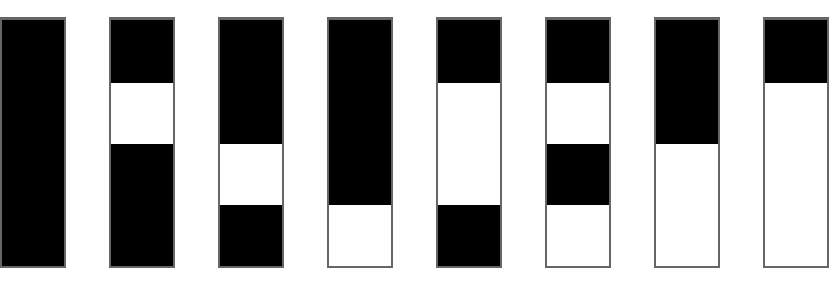
\includegraphics[height=2.5cm]	{1qubit_PCEOperations}
		\caption{}
		\label{fig:PCE_figs_examples_a}
	\end{subfigure}
	\hfill
	\begin{subfigure}[b]{0.48\textwidth}
		\centering
		\hfill 
		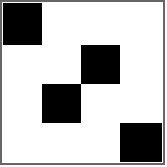
\includegraphics[height=2.3cm]{2qubits_pceChannel_example01} 
		\hfill
		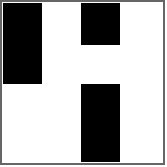
\includegraphics[height=2.3cm]{2qubits_pce_example}		
		\hfill \hfill
		\caption{}
		\label{fig:PCE_figs_examples_b}
	\end{subfigure}
	\newline
	\begin{subfigure}[c]{0.6\textwidth}
		\centering
		\vspace{-.7cm}
		\hspace*{\fill}
		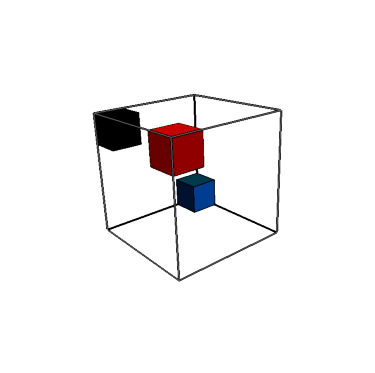
\includegraphics[width=4cm]{3qubits_PCE_ex1}
		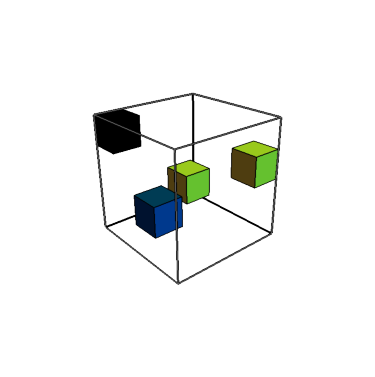
\includegraphics[width=4cm]{3qubits_PCE_ex2}
		\hspace*{\fill}
		\vspace{-.7cm}
		\caption{}
		\label{fig:PCE_figs_examples_c}
	\end{subfigure}
%	\begin{subfigure}[b]{0.38\textwidth}
%		\centering
%		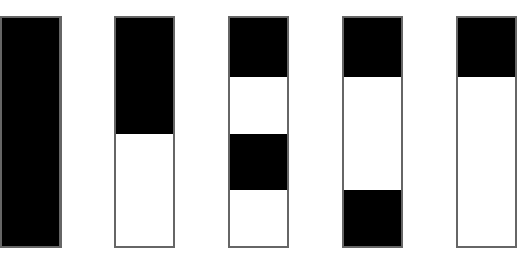
\includegraphics[height=2.5cm]	{1qubit_PCEChannels}
%		\caption{}
%		\label{fig:PCE_figs_examples_a}
%	\end{subfigure}
	\caption{\textbf{(a)} Figuras PCE de todas las operaciones PCE de 1 qubit. 
	\textbf{(b)} Figuras PCE de 2 operaciones PCE de 2 qubits aleatorias. La primera 
	figura PCE representa a un canal PCE y la segunda representa una operación 
	PCE que no satisface la condición de completa positividad. 
	\textbf{(c)} Figuras PCE de dos operaciones PCE aleatorias de 3 qubits. \ep}
	\label{fig:PCE_figs_examples}
\end{figure} % }}}

%\noindent
%\esqueleto{En este punto, ya es más o menos obvio cómo es la representación 
%geométrica de 3 qubits y que a partir de 4 qubits ya no podremos utilizar 
%esta herramienta geométrica. Mostrar algunas figuras de PCEs de 3 qubits
%y hablar de cómo hacer diferencia entre correlaciones y componentes 
%locales en esas figuras según los colores 
%(sólo para 3 qubits, porque las de 1 y 2 qubits 
%las voy a poner en negro).}

La representación de las figuras PCE puede utilizarse para representar 
operaciones PCE hasta de 3 qubits. En este punto, esta afirmación puede 
ser más o menos obvia, pero es importante dejar claro las limitaciones de 
la representación de las figuras PCE. 
Ya que los índices $j_1,\ldots,j_n$ están asociados a las posiciones 
en las figuras PCE, entonces se necesita una figura $n$ dimensional para representar 
a una operación PCE de $n$ qubits. Por lo tanto, las figuras PCE pueden
utilizarse sólo para representar operaciones PCE de 1, 2 y 3 qubits. 

%\noindent
%\esqueleto{Armados con esta potente herramienta geométrica, ahora 
%es mucho más sencillo ganar intuición de las operaciones PCE e inferir 
%características de los canales PCE. Entonces ahora mostraré los resultados 
%de la sección anterior, pero usando las figuritas.}

Ahora que ya introdujimos y discutimos la representación de las figuras PCE,
vamos a utilizar esta nueva representación para presentar otra vez 
los resultados de las Tablas \ref{tab:2qubitsPCEChannel1sAnd0s} 
y \ref{tab:3qubitsPCEChannel1sAnd0s} de los canales PCE de 2 y 
parcialmente de 3 qubit.
En la \Fref{fig:2qubits_PCEChannels_figs} se muestran los canales cuánticos PCE de 2 qubits. 
En la \Fref{fig:3qubits_PCEChannels_figs} 
mostramos sólo canales cuánticos PCE de 3 qubits representativos. En la siguiente 
sección vamos a discutir detenidamente a qué nos referimos por representativos.
No colocamos todas las figuras PCE de los canales PCE de 3 qubits que 
encontramos porque ocuparían demasiadas páginas.
En contraste con las listas de 1's y 0's, las figuras PCE proporcionan mucha 
más intuición de que sí existen características en común de los canales 
cuánticos PCE, como los patrones tan particulares que se obervan en la
\Fref{fig:2qubits_PCEChannels_figs}. En la siguiente y última sección 
de este capítulo, vamos a discutir en profundidad la caracterización de los 
canales cuánticos PCE que se evidencian en nuestros resultados de 2 y 3 qubits.

\janote{Me tocó poner \texttt{[H]} 
en los siguientes dos entornos \texttt{figure} porque de lo contrario, 
las figuras se iban hasta el final del capítulo, después de la última sección.}
%\newpage
\begin{figure}[H]
\centering
\begin{minipage}[t]{0.49\textwidth}
	\centering
		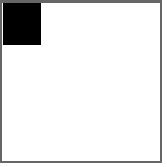
\includegraphics[height=1.4cm]{C1}
		\subcaption{C$\subind{1}{}$}
	\end{minipage} \\ \vspace{.25cm} 
	\begin{minipage}[b]{0.49\textwidth}
		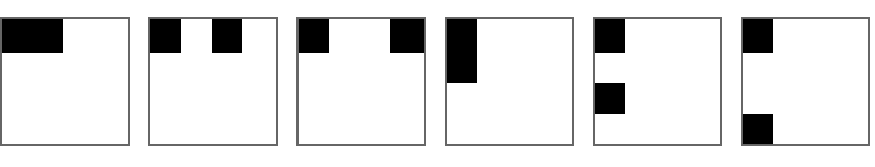
\includegraphics[height=1.4cm]{C2_1}
		\subcaption{C$\subind{2}{1}$}
	\end{minipage} \hfill
	\begin{minipage}[b]{0.49\textwidth}
		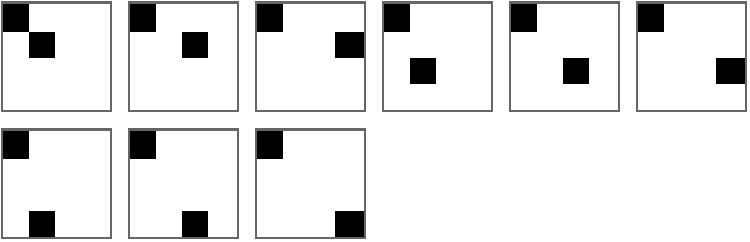
\includegraphics[height=2.4cm]{C2_2}
		\subcaption{C$\subind{2}{2}$}
	\end{minipage} \\ \vspace{.25cm} 
	\begin{minipage}[b]{0.49\textwidth}
		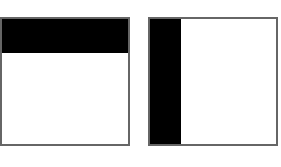
\includegraphics[height=1.4cm]{C4_1}
		\subcaption{C$\subind{4}{1}$}
	\end{minipage} \hfill
	\begin{minipage}[b][3.1cm]{0.49\textwidth}
		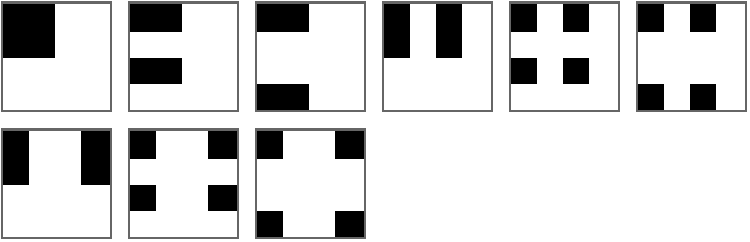
\includegraphics[height=2.4cm]{C4_2}
		\subcaption{C$\subind{4}{2}$}
	\end{minipage} \\ \vspace{-.5cm} 
	\begin{minipage}[b]{0.49\textwidth}
		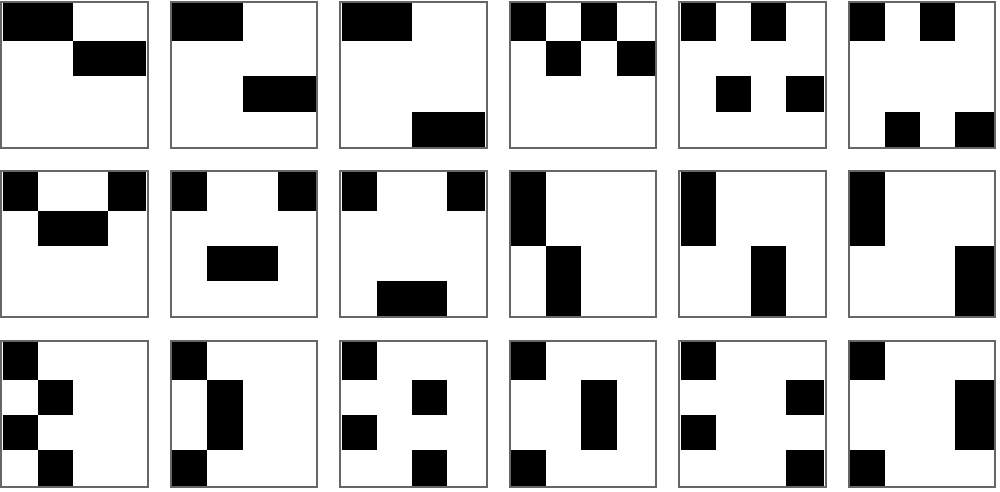
\includegraphics[height=3.6cm]{C4_3}
		\subcaption{C$\subind{4}{3}$}
		\label{fig:C_4^3}
	\end{minipage} \hfill
	\begin{minipage}[b][5.1cm]{0.49\textwidth}
		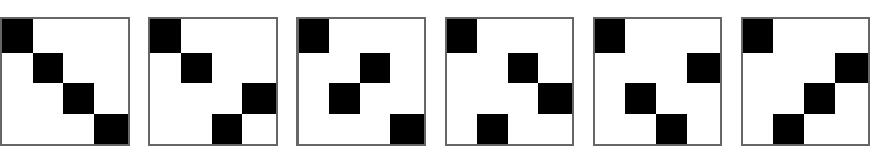
\includegraphics[height=1.4cm]{C4_4}
		\subcaption{C$\subind{4}{4}$}
	\end{minipage} \\ \vspace{-1.9cm} 
	\begin{minipage}[b]{0.49\textwidth}
		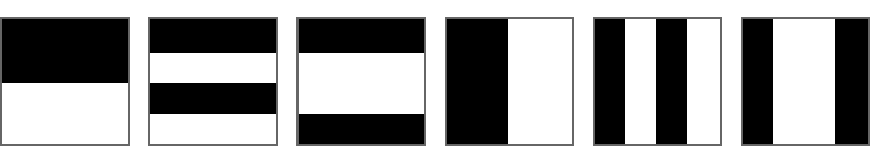
\includegraphics[height=1.4cm]{C8_1}
		\subcaption{C$\subind{8}{1}$}
	\end{minipage} \hfill
	\begin{minipage}[b][5.1cm]{0.49\textwidth}
		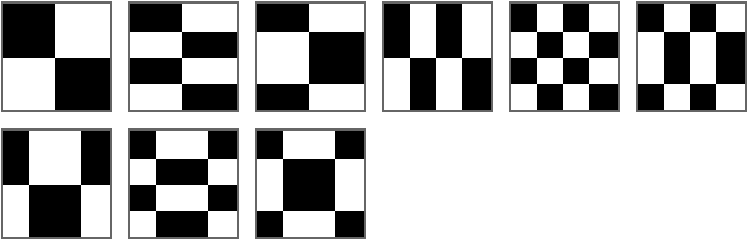
\includegraphics[height=2.4cm]{C8_2}
		\subcaption{C$\subind{8}{2}$}
		\label{fig:C_8^2}
	\end{minipage} \\	\vspace{.5cm} 
	\begin{minipage}[b]{0.49\textwidth}
	\centering
		
\includegraphics[height=1.4cm]{C16}
		\subcaption{C$\subind{16}{}$}
	\end{minipage}
	\caption{Figuras PCE de los canales cuánticos PCE de 2 qubits ordenados por 
	clases de equivalencia etiquetadas como C$\subind{k}{l}$, donde $k$ es el número 
	de componentes de Pauli invariantes y $l$ es para diferenciar entre clases 
	de equivalencia con el mismo número de componentes de Pauli invariantes.
	Los elementos de una misma clase de equivalencia están conectados por 
	intercambios de partículas y permutaciones locales de base. \ep}
	\label{fig:2qubits_PCEChannels_figs}
\end{figure} 
\begin{figure}[H]
	\centering
	\vspace{-.5cm}
	\begin{minipage}[t]{.9\textwidth}
		\centering
		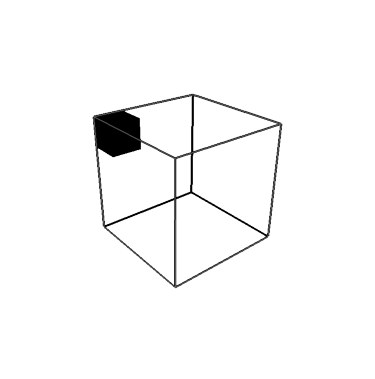
\includegraphics[width=4cm]{3q_0}
		\vspace{-.5cm} 
		\subcaption{Figura PCE del único canal cuántico PCE de 3 qubits que deja invariante 
		sólo 1 componente de Pauli.}
		\vspace{-.5cm}
	\end{minipage}
	\begin{minipage}[t]{.9\textwidth}
		\centering
		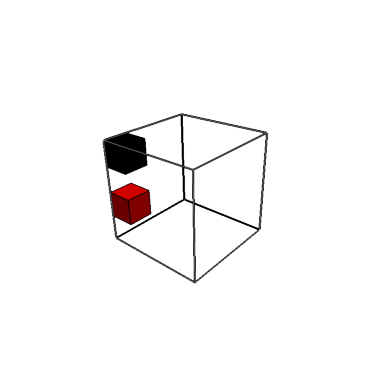
\includegraphics[width=4cm]{3q_2c_1} \hfill
		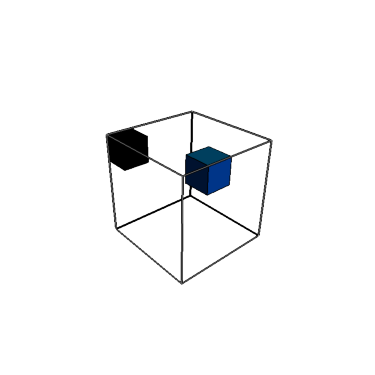
\includegraphics[width=4cm]{3q_2c_2} \hfill
		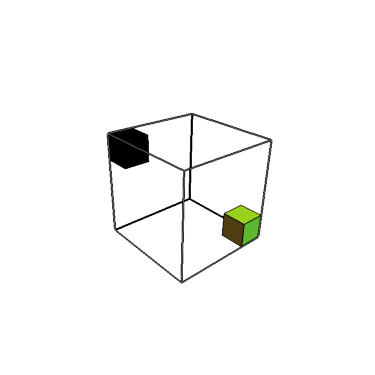
\includegraphics[width=4cm]{3q_2c_3}
		\vspace{-.5cm} 
		\subcaption{Figuras PCE de un canal cuántico PCE de cada una 
		de las 3 clases de equivalencia de los canales cuánticos PCE de 3 qubits
		 que dejan invariantes 2 componentes de Pauli.}
		 \vspace{-.5cm}
	\end{minipage}
	\begin{minipage}[t]{.9\textwidth}
		\centering
		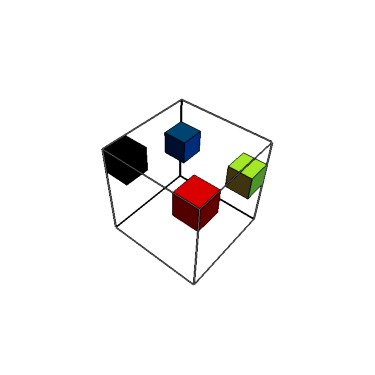
\includegraphics[width=4cm]{3q_5} \hfill
		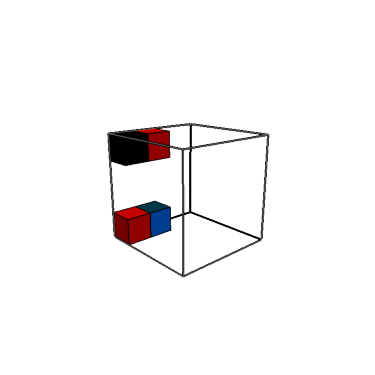
\includegraphics[width=4cm]{3q_8} \hfill
		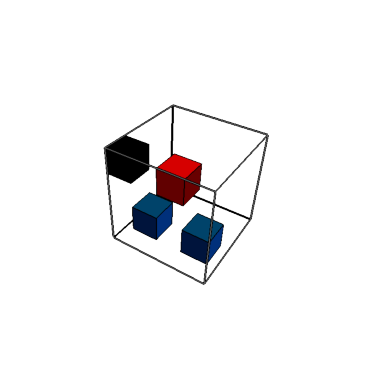
\includegraphics[width=4cm]{3q_1} \\ \vspace{-1cm} 
		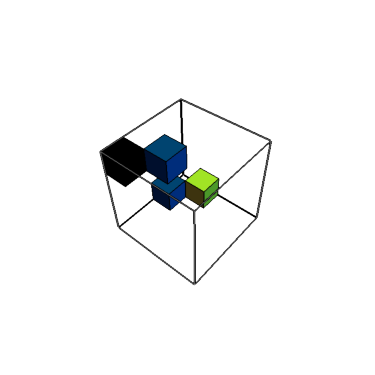
\includegraphics[width=4cm]{3q_2} \hfill
		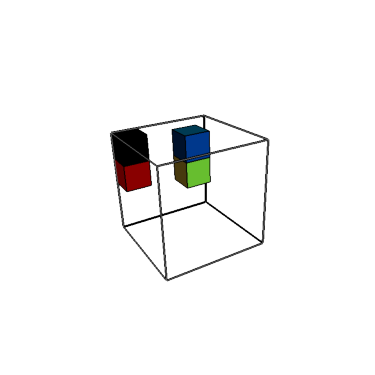
\includegraphics[width=4cm]{3q_9} \hfill
		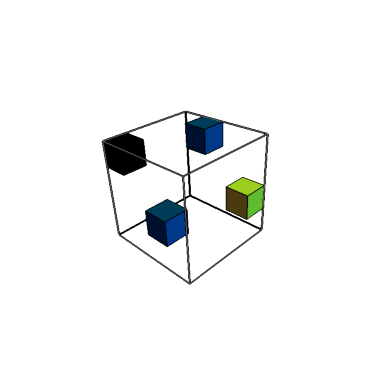
\includegraphics[width=4cm]{3q_4}  \\ \vspace{-1cm} 
		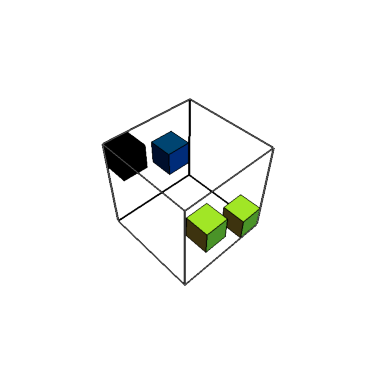
\includegraphics[width=4cm]{3q_6} \hfill
		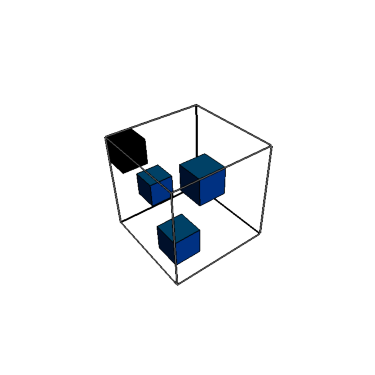
\includegraphics[width=4cm]{3q_3} \hfill
		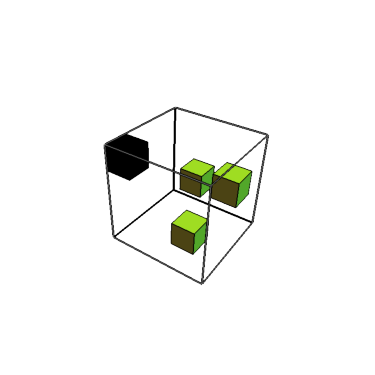
\includegraphics[width=4cm]{3q_7} 
		\vspace{-.5cm} 
		\subcaption{Figuras PCE de un canal cuántico PCE de cada una 
		de las 9 clases de equivalencia de los canales cuánticos PCE de 3 qubits
		 que dejan invariantes 4 componentes de Pauli.}
	\end{minipage}
	\begin{minipage}[t]{.9\textwidth}
		\centering
		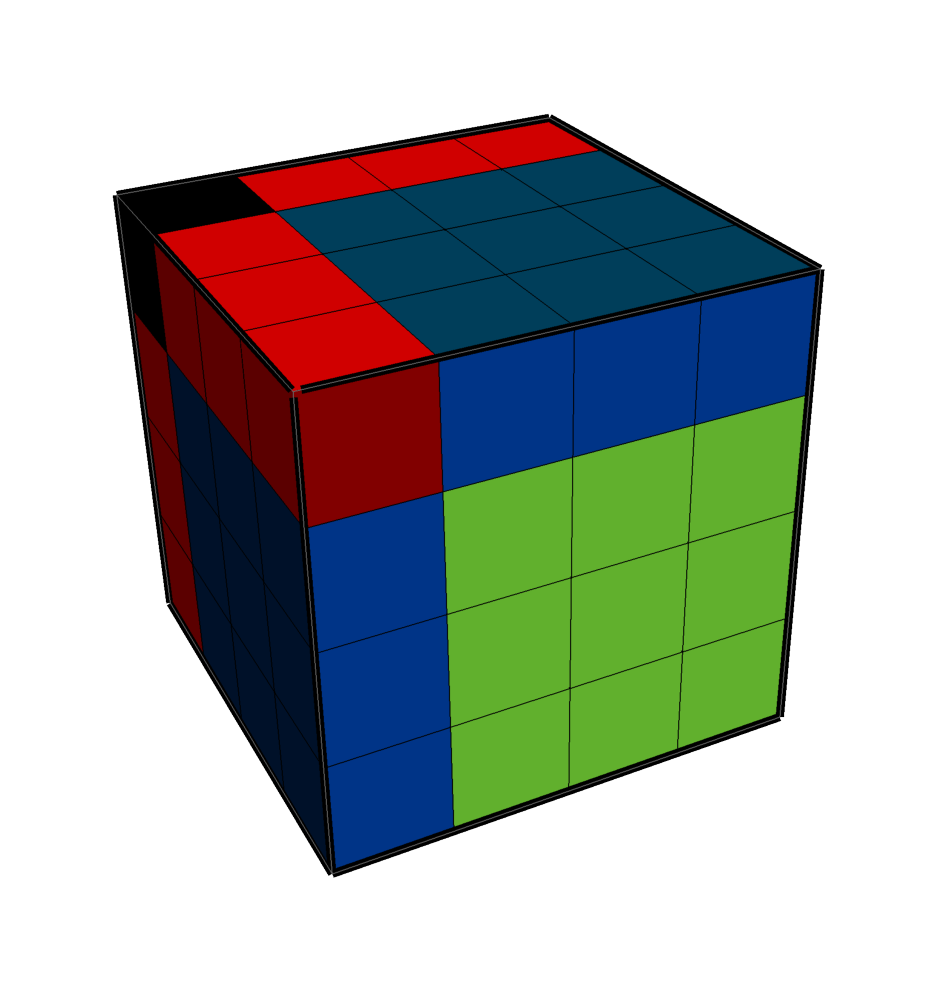
\includegraphics[width=2.2cm]{cubo_3qubits}
		\subcaption{Figura PCE de la operación identidad, un canal cuántico 
		PCE que deja invariantes 64 componentes de Pauli.}
	\end{minipage}
	\caption{Figuras PCE de los canales cuánticos PCE de 3 qubits. \ep}
	\label{fig:3qubits_PCEChannels_figs}
\end{figure}

\section{Discusión de resultados}\label{sec:ch3_discussion}
\janote{Con el fin de hacer más eficiente la redacción, voy a partir del 
documento que preparamos para Sergey (justo coincide los resultados
que iban ahí con lo que vamos a poner en la tesis) y voy a iterar.}

\esqueleto{Esta sección es la que posee el contenido más importante 
de este manuscrito, después de la motivación y planteamiento del 
problema. Después de esta sección, lo único que haremos será 
estudiar si las operaciones PCE son un subconjunto de otras operaciones 
que fueron estudiadas por Ruskai.}

Intro de la sección: la escribiré al terminar de redactar la sección.

\esqueleto{Existen familias de canales PCE equivalentes. En las figuritas, 
esto se ve como transposiciones y permutaciones de filas y columnas. 
Físicamente, estos son swaps de partículas y cambios de base local.
Aquí yo creería que vale la pena discutir en palabritas, como en el documento
para sergey, pero también echarle algunas expresiones matemáticas como 
la de aplicar un swap, el PCE, y otro swap, por ejemplo...}

Los canales PCE pueden clasificarse en clases de equivalencia (como 
mostramos en las Figs. \ref{fig:2qubits_PCEChannels_figs} y 
\ref{fig:3qubits_PCEChannels_figs}). 
Los canales PCE pueden clasificarse en subconjuntos dentro los cuales todos 
los elementos son equivalentes bajo dos operaciones diferentes. 
Nuestros resultados muestran que los canales PCE que pertenecen a 
una misma clase de equivalencia están conectados vía 
\begin{enumerate}
	\item Intercambios de partículas. Los qubits en un sistema pueden 
	intercambiarse. Por lo tanto, si una operación PCE es un canal cuántico 
	para alguna configuración de los qubits en el sistema, entonces existen canales 
	PCE equivalentes que actúan sobre todas las posibles configuraciones 
	de qubits de un sistema. En las figuras PCE de los canales PCE de 2 qubits 
	de la \Fref{fig:2qubits_PCEChannels_figs} 
	se puede visualizar esta equivalencia como transposiciones. A continuación,
	como un ejemplo, 
	mostramos cuál es el canal PCE equivalente, mediante intercambio
	de partículas, del primer elemento de C${}_4^3$ en la \Fref{fig:C_4^3}.
	\begin{center}
	\begin{tabular}{P{2cm} P{1.5cm} P{2cm}}
		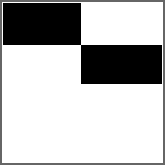
\includegraphics[width=2cm]{particle_swap_1}
		& \hspace*{\fill} $\stackrel{T}{\longmapsto}$ \hspace*{\fill}
		& 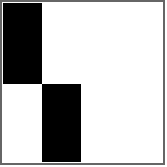
\includegraphics[width=2cm]{particle_swap_2}
	\end{tabular}
	\end{center}
	
	\item Intercambio de etiquetas de los ejes\janote{permutaciones de elementos de una base local}. Estas operaciones corresponden 
	a permutaciones de filas y/o columnas en las figuras PCE de 2 qubits 
	en \Fref{fig:2qubits_PCEChannels_figs}. En general, la permutación de los 
	elementos $\sigma_1^{(i)},\sigma_2^{(i)}$ y $\sigma_3^{(i)}$ de la 
	base local de la $i$-ésima partícula del sistema resulta en una \janote{rotación} 
	de la esfera de Bloch de la $i$-ésima particula. Veamos abajo un 
	ejemplo del canal PCE equivalente del primer elemento de C${}_8^2$
	en la \Fref{fig:C_8^2} cuando se hace la transformación
	$\{\sigma_0^{(2)},\sigma_1^{(2)},\sigma_2^{(2)},\sigma_3^{(2)}\}\mapsto
	\{\sigma_0^{(2)},\sigma_3^{(2)},\sigma_1^{(2)},\sigma_2^{(2)}\}$
	a la base local del qubit 2.
	\begin{center}
	\begin{tabular}{P{2cm} P{1.5cm} P{2cm}}
		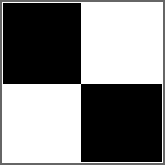
\includegraphics[width=2cm]{permutation_1}
		& \hspace*{\fill} $\longmapsto$ \hspace*{\fill}
		& 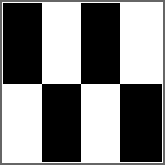
\includegraphics[width=2cm]{permutation_2}
	\end{tabular}
	\end{center}
\end{enumerate}
Si bien hemos enunciado ejemplos de canales PCE de 2 qubits para 
proporcionar intuición al lector, no debe olvidarse que nuestros resultados 
muestran que los canales PCE de 1, 2 y 3 qubits pueden clasificarse 
según las operaciones de intercambios de partículas y de etiquetas de los ejes.
Lo cual, es evidencia numérica de una clasificación general que se puede aplicar 
a los canales PCE de sistemas de $n$ qubits. 

\esqueleto{Las figuras de los canales PCE exhiben patrones que todos 
comparten, parecen respetar alguna simetría...}

\esqueleto{Todos los canales PCE obedecen la regla de $2^k$...}

\esqueleto{Hay correspondencia en el número de canales PCE que 
dejan $2^k$ y $2^{2n-k}$ componentes de Pauli invariantes.} \janote{jm?}

\esqueleto{Amarrado a la correspondencia de ``arcoiris'' van las reglas 
empíricas que formulamos con Alejo. Esta es otra prueba empírica que 
respalda la hipótesis de una conexión/correspondencia entre canales PCE.}

En general, nuestros resultados numéricos exhiben las siguientes 
propiedades de los canales PCE:
\begin{enumerate}
	\item \textit{(Regla $2^k$)} Los canales PCE dejan invariantes una cantidad 
	que es potencia de 2 de componentes de Pauli. No obstante, la regla $2^k$
	no es la única que determina que una operación PCE sea completamente
	positiva. Es decir, existen operaciones PCE que dejan invariantes $2^k$
	componentes de Pauli que no son canales cuánticos, como es el caso 
	de la operación PCE de la figura PCE que mostramos abajo. Esta operación 
	PCE deja invariantes 4 $(2^2)$ componentes de Pauli, pero no satisface 
	la completa positividad y, por consiguiente, no es un canal cuántico.
	\begin{center}
		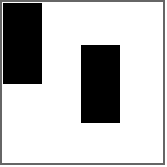
\includegraphics[width=2cm]{badPCE}
	\end{center}
	
	\item \textit{(Regla espejo)} El número de canales PCE de $n$ qubits 
	como función de 	los exponentes $k$, del número $2^k$ de componentes de Pauli 
	invariantes, es simétrico respecto a $n$. En la \Fref{fig:mirroring} mostramos 
	las gráficas de el número de canales PCE de 1, 2 y 3 qubits 
	en función del exponente $k$ del número $2^k$
	de componentes de Pauli que dejan invariantes. Nótese la simetría respecto a 
	$k=n$ en las gráficas de las Figs. \ref{fig:mirroring_1qubit} y 
	\ref{fig:mirroring_2qubits}. Es, a partir de estos resultados, que suponemos 
	que los puntos en azul de la gráfica de la \Fref{fig:mirroring_3qubits}
	también existen para que la gráfica también sea simétrica respecto a $k=3$.
	\begin{figure} % {{{
	\centering
	\begin{subfigure}[b]{0.48\textwidth}
		\centering
		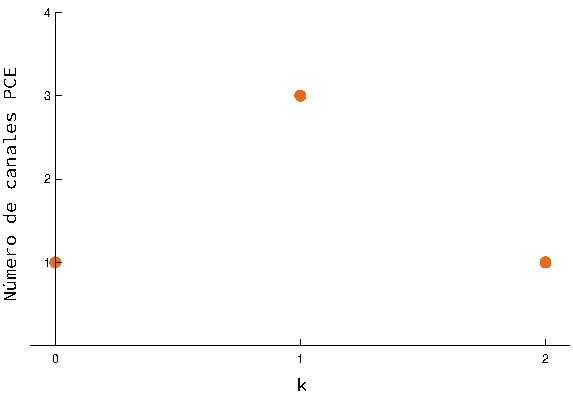
\includegraphics[width=7cm]	{mirroring_1qubits}
		\caption{}
		\label{fig:mirroring_1qubit}
	\end{subfigure}
	\hfill
	\begin{subfigure}[b]{0.48\textwidth}
		\centering
		\hfill 
		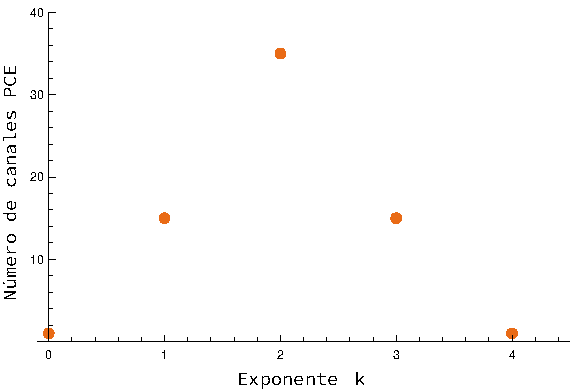
\includegraphics[width=7cm]{mirroring_2qubits} 
		\hfill \hfill
		\caption{}
		\label{fig:mirroring_2qubits}
	\end{subfigure}
	\newline
	\begin{subfigure}[c]{\textwidth}
		\centering
		\hspace*{\fill}
		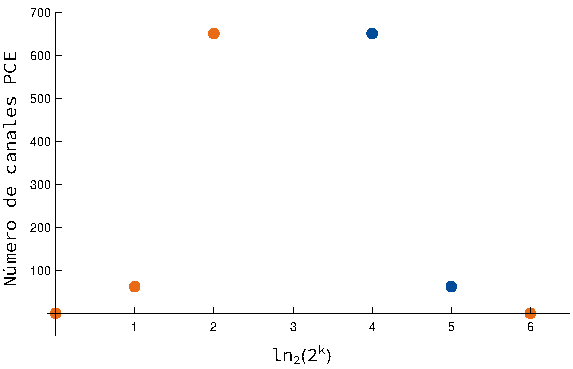
\includegraphics[width=7cm]{mirroring_3qubits}
		\hspace*{\fill}
		\caption{}
		\label{fig:mirroring_3qubits}
	\end{subfigure}
	\caption{Gráficas del número de canales PCE de 1, 2 y 3 qubits
	en función del exponente $k$ 	del número $2^k$ 	de componentes 
	de Pauli invariantes que dejan 	invariantes los canales. \textbf{(a)} 1 qubit. 
	\textbf{(b)} 2 qubits. \textbf{(c)} 3 qubits. Los puntos en azul representan 
	los casos no explorados 	con nuestro método numérico, pero que suponemos 
	por la regla de espejo	que existen. \ep}
	\label{fig:mirroring}
\end{figure} % }}}
\end{enumerate}
Como una consecuencia de los sistemas multipartitos la acción de
un canal PCE sobre cada subsistema debe ser otro canal PCE. Esto puede 
interpretarse en las figuras PCE de la siguiente forma. En todas las figuras PCE
de la \Fref{fig:2qubits_PCEChannels_figs} debe tenerse canales PCE de 1 qubit 
en la primera fila y en la primera columna, que representan la acción del 
canal cuántico de 2 qubits sobre las componentes locales de cada uno de los dos 
qubits. Por ejemplo, la operación que representa la figura PCE de abajo, aunque 
cumple la regla $2^k$, no puede ser un canal cuántico porque la acción 
sobre el qubit 1 (primera fila) no es un canal cuántico. Sabemos que 
una operación PCE de 1 qubit que deja invariantes 3 componentes de Pauli
no satisface la completa positividad (ver \Tref{tab:1qubit_PCE} y \Fref{fig:PCE_figs_examples}).
\begin{center}
	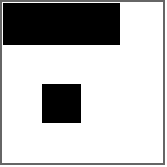
\includegraphics[width=2cm]{badPCE1}
\end{center}

\esqueleto{La familia más sencilla de analizar es la de los PCE de 1 qubit
que dejan dos componentes de Pauli invariantes. Todos se pueden entender 
como la misma operación, pero conectados por rotaciones.}

Vamos ahora, a partir de observaciones empíricas de las figuras PCE 
de los canales PCE de 2 qubits (ver \Fref{fig:2qubits_PCEChannels_figs}) 
y de las propiedades que recién mencionamos, a discutir 
cómo construir canales PCE de 2 qubits utilizando sólo la representación
de las figuras PCE.
\begin{enumerate}
	\item Consideramos el canal PCE con $\tau_{00}=1$ y el resto de elementos
	iguales a cero. Podemos construir cualquiera de los canales PCE 
	de 2 componentes de Pauli invariantes escogiendo cualquiera del resto de 
	$\tau_{ij}$ igual a 1. 
	\begin{enumerate}
		\item Escoger un elemento de la forma $\tau_{k 0}=1$. Supongamos, 
		para ejemplificar, que escogemos $\tau_{20}=1$. Tenemos entonces 
		el canal PCE: 
		\begin{center}
			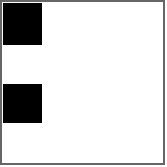
\includegraphics[width=2cm]{11}
		\end{center}
		Para construir 
		ahora otro canal PCE, pero ahora de 4 componentes de Pauli invariantes, hay
		dos bifurcaciones según la selección de $\tau_{ij}$ iguales a 1:
		\begin{enumerate}
			\item Escoger $\tau_{km}=\tau_{0m}=1$, con $m\in\{1,2,3\}$.
			Siguiendo nuestro ejemplo, tendríamos el canal PCE:
			\begin{center}
				
\includegraphics[width=2cm]{111}
			\end{center}
			\item Escoger $\tau_{m_1l}=\tau_{m_2l}=1$, con 
			$\{m_1,m_2\}= \{1,2,3\}\backslash\{k\}$ y $l\in \{1,2,3\}$. 
			Siguiendo nuestro ejemplo y si escogemos $l=3$:
			\begin{center}
				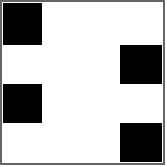
\includegraphics[width=2cm]{112}
			\end{center}
		\end{enumerate}
		
		\item Escoger $\tau_{km}=\tau_{k0}=\tau_{0m}=1$ con $k,m\in\{1,2,3\}$.
		Partimos, una vez más del ejemplo propuesto en 1.1 y escogemos $m=3$:
		\begin{center}
				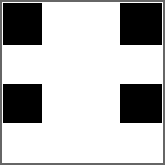
\includegraphics[width=2cm]{12}
			\end{center}
	\end{enumerate}
	Nótese que los canales PCE que se construyen en 1.1.1 y 1.2 son canales 
	que pertenecen a la misma clase de equivalencia.

	\item Supongamos que partimos de un canal PCE construído con las reglas 
	del item 1.1.1, es decir un canal PCE con 
	$\tau_{00}=\tau_{kl}=\tau_{k0}=\tau_{0l}=1$.
	Podemos construir ahora un canal PCE de 8 componentes de Pauli invariantes si 
	escogemos algunas de las siguientes dos opcionesm
	\begin{enumerate}	
	\item $\tau_{m_1,0}=\tau_{m_2,0}=\tau_{m_1,l}=\tau_{m_2,l}=1$
	con $\{m_1,m_2\}= \{1,2,3 \}\backslash\{k \}$. Continuando el ejemplo de 1.1.1, 
	esto nos lleva al siguiente canal PCE:
	\begin{center}
				
\includegraphics[width=2cm]{21}
			\end{center}
	\item $\tau_{m_1,0}=\tau_{m_2,0}=\tau_{k,m_1}=\tau_{k,m_2}=1$
	con $\{m_1,m_2\}=\{1,2,3 \}\backslash\{l \}$. Una última vez, del ejemplo 
	del canal PCE en 1.1.1, esta regla nos conduce a:
	\end{enumerate}
	\begin{center}
			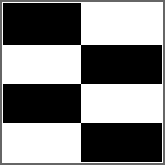
\includegraphics[width=2cm]{22}
	\end{center}
	Podríamos discutir cuáles son las reglas construir un canal PCE de 8 componentes 
	de Pauli invariantes a partir de un canal generado en el item 1.1.2, pero no es 
	necesario, pues los canales PCE construidos con las reglas en 2.1 y 2.2 es 
	suficiente para encontrar el resto de canales PCE de 8 componentes de Pauli 
	invariantes mediante intercambios de partículas y de etiquetas de los ejes.
\end{enumerate}
Con esta conjunto de reglas empíricas es posible construir todos
los canales PCE de 2 qubits, excepto la los canales que pertenecen
a la clase de equivalencia C${}_4^4$. Reglas empíricas similares pueden 
observarse para los canales PCE de 3 qubits, pero no vale la pena discutirlo.
De hecho, el objetivo de discutir las reglas empíricas observadas para los 
canales PCE de 2 qubits es para hacer remarcar, a partir de las figuras PCE,
los indicios de una estructura matemática que obedecen los canales PCE. 

\esqueleto{Listo, hagamos un resumen de las características puntuales 
que inferimos de los canales PCE: ta ta ta.... Ahora sólo nos hace falta 
formalizar todo esto y hacer conexión formal entre todas las características. 
Además, sería deseable buscar alternativas para poder 
explorar numéricamente el caso completo de 3 e incluso de 4 qubits.}